

\tikzset{every picture/.style={line width=0.75pt}} %set default line width to 0.75pt        

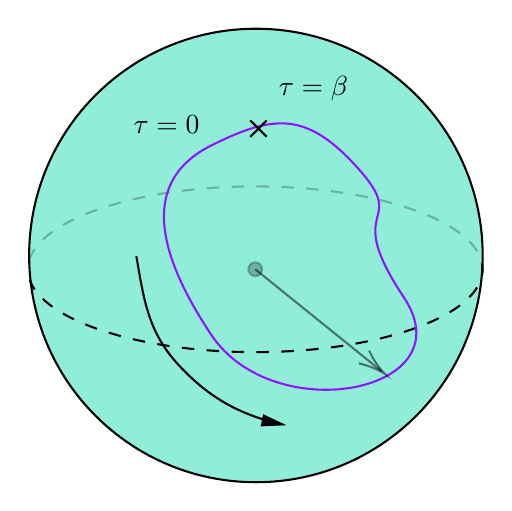
\begin{tikzpicture}[x=0.75pt,y=0.75pt,yscale=-1,xscale=1]
%uncomment if require: \path (0,300); %set diagram left start at 0, and has height of 300

%Shape: Circle [id:dp4271001416525375] 
\draw  [fill={rgb, 255:red, 80; green, 227; blue, 194 }  ,fill opacity=0.64 ] (100.21,156.46) .. controls (100.21,96.12) and (149.12,47.21) .. (209.46,47.21) .. controls (269.79,47.21) and (318.71,96.12) .. (318.71,156.46) .. controls (318.71,216.79) and (269.79,265.71) .. (209.46,265.71) .. controls (149.12,265.71) and (100.21,216.79) .. (100.21,156.46) -- cycle ;
%Shape: Arc [id:dp5416427461491542] 
\draw  [draw opacity=0][dash pattern={on 4.5pt off 4.5pt}] (318.45,160.4) .. controls (318.62,161.29) and (318.7,162.19) .. (318.7,163.09) .. controls (318.7,185.14) and (269.66,203.02) .. (209.16,203.03) .. controls (153.32,203.04) and (107.23,187.82) .. (100.46,168.14) -- (209.15,163.11) -- cycle ; \draw  [dash pattern={on 4.5pt off 4.5pt}] (318.45,160.4) .. controls (318.62,161.29) and (318.7,162.19) .. (318.7,163.09) .. controls (318.7,185.14) and (269.66,203.02) .. (209.16,203.03) .. controls (153.32,203.04) and (107.23,187.82) .. (100.46,168.14) ;
%Shape: Arc [id:dp27514417350783926] 
\draw  [draw opacity=0][dash pattern={on 4.5pt off 4.5pt}] (318.45,165.82) .. controls (318.62,164.93) and (318.7,164.03) .. (318.7,163.13) .. controls (318.7,141.08) and (269.66,123.2) .. (209.16,123.19) .. controls (153.32,123.18) and (107.23,138.4) .. (100.46,158.08) -- (209.15,163.11) -- cycle ; \draw  [color={rgb, 255:red, 0; green, 0; blue, 0 }  ,draw opacity=0.25 ][dash pattern={on 4.5pt off 4.5pt}] (318.45,165.82) .. controls (318.62,164.93) and (318.7,164.03) .. (318.7,163.13) .. controls (318.7,141.08) and (269.66,123.2) .. (209.16,123.19) .. controls (153.32,123.18) and (107.23,138.4) .. (100.46,158.08) ;
%Shape: Polygon Curved [id:ds05822553982795253] 
\draw  [color={rgb, 255:red, 144; green, 19; blue, 254 }  ,draw opacity=1 ] (187.96,103.47) .. controls (218.36,88.26) and (234.23,87.07) .. (258.97,114.83) .. controls (283.71,142.58) and (250.3,130.97) .. (280.71,176.58) .. controls (311.11,222.2) and (218.36,240.31) .. (187.96,194.69) .. controls (157.55,149.08) and (157.55,118.67) .. (187.96,103.47) -- cycle ;
%Straight Lines [id:da6134231895751854] 
\draw [color={rgb, 255:red, 0; green, 0; blue, 0 }  ,draw opacity=1 ]   (210.68,95.34) ;
\draw [shift={(210.68,95.34)}, rotate = 45] [color={rgb, 255:red, 0; green, 0; blue, 0 }  ,draw opacity=1 ][line width=0.75]    (-5.59,0) -- (5.59,0)(0,5.59) -- (0,-5.59)   ;
%Straight Lines [id:da9066706253629926] 
\draw [color={rgb, 255:red, 0; green, 0; blue, 0 }  ,draw opacity=0.5 ][line width=0.75]    (270.15,212.33) -- (209.15,163.11) ;
\draw [shift={(271.71,213.58)}, rotate = 218.9] [color={rgb, 255:red, 0; green, 0; blue, 0 }  ,draw opacity=0.5 ][line width=0.75]    (13.12,-3.95) .. controls (8.34,-1.68) and (3.97,-0.36) .. (0,0) .. controls (3.97,0.36) and (8.34,1.68) .. (13.12,3.95)   ;
%Straight Lines [id:da5443690821222467] 
\draw    (100,149.66) ;
%Straight Lines [id:da23851388151552166] 
\draw [color={rgb, 255:red, 0; green, 0; blue, 0 }  ,draw opacity=0.25 ]   (209.15,163.11) ;
\draw [shift={(209.15,163.11)}, rotate = 0] [color={rgb, 255:red, 0; green, 0; blue, 0 }  ,draw opacity=0.25 ][fill={rgb, 255:red, 0; green, 0; blue, 0 }  ,fill opacity=0.25 ][line width=0.75]      (0, 0) circle [x radius= 3.35, y radius= 3.35]   ;
%Curve Lines [id:da94729558266777] 
\draw    (151.85,156.78) .. controls (155.41,177.15) and (157.29,192.83) .. (171.61,208.56) .. controls (185.57,223.89) and (200.71,233.21) .. (222.42,237.89) ;
\draw [shift={(224.11,238.24)}, rotate = 191.4] [fill={rgb, 255:red, 0; green, 0; blue, 0 }  ][line width=0.08]  [draw opacity=0] (12,-3) -- (0,0) -- (12,3) -- cycle    ;

% Text Node
\draw (149,87.4) node [anchor=north west][inner sep=0.75pt]    {$\tau =0$};
% Text Node
\draw (219,68.4) node [anchor=north west][inner sep=0.75pt]    {$\tau =\beta $};


\end{tikzpicture}
